% !TEX encoding = UTF-8 Unicode
\section{Resoconto delle varie attività di verifica}
		\subsection{Fase A}
			\subsubsection{Documenti}
				\paragraph{Verifiche manuali}
					Durante questa fase sono stati verificati i documenti seguendo le procedure presenti nella sezione Verifica nel documento \insdoc{Norme di Progetto}.\\\\
					É stata quindi applicata un'analisi  statica di tutti i documenti con lo scopo di rilevare errori di struttura, forma e contenuto in esso contenuti. Poichè in questa fase iniziale i documenti dovevano ancora essere verificati interamente, si è proceduto con una verifica di tipo \textit{walkthrough}. Durante questa attività sono emersi alcuni errori che sono stati segnalati. Si è quindi cercato di capire il problema e di trovarne una soluzione, per poi passare alla sua correzione.\\ \\%nelle prossime fasi verificherò solo dove sono avvenute modifiche quindi un controllo semi-mirato
					In questa prima fase sono stati nuovamente analizzati attraverso \textit{walkthrough} tutti i documenti alla ricerca dei termini che dovrebbero essere inclusi nel \insdoc{Glossario} ma che ancora non lo erano. Trovati, sono stati quindi segnalati e di conseguenza aggiunti. Da questa attività sono stati segnalati 7 termini, ma gli \insrole{Amministratori} hanno ritenuto più opportuno aggiungere solamente 5 di essi al \insdoc{Glossario} .\\\\
					Vengono poi analizzati anche i diagrammi dei casi d'uso cercando di capire se i vari attori erano davvero tali. Si è fatto riferimento alla sezione 6.2.2.1 del documento \insdoc{Norme di Progetto}. Non sono stati rilevati problemi di questo genere.\\\\
					É stato quindi verificato che per ogni diagramma siano state utilizzate secondo lo standard UML le relazioni di inclusione, generalizzazione ed estensione. Nemmeno da questa verifica sono emersi errori.\\\\
					Sono stati infine valutate le descrizioni dei casi d'uso con lo scopo di assicurarsi che sia stato descritto cosa il sistema fa e non cosa non fa. Anche questa verifica si è conclusa positivamente.
				\paragraph{Verifiche automatizzate}
					Gli strumenti utilizzati per la verifica automatica dei documenti si trovano nella sezione 6.3 del documento \insdoc{Norme di Progetto}.\\\\
					É stato sfruttato lo script \textit{OrtographicCheck} per  il controllo ortografico di tutti i documenti. Esso ha evidenziato alcuni errori di battitura che sono stati subito corretti.\\\\
					É stato poi eseguito lo script \textit{Gulpease} per calcolare l'indice di leggibilità di ogni documento. Di seguito si riportano, in formato tabellare, gli esiti ritornati dallo script.
					\begin{table}[H]\centering
						\begin{tabu}{| l | c | c |}
							\hline
							Documenti 				& Gulpease	& Esito  \\ \hline
							
							Norme di Progetto 				& 57		& Superato 		 \\
							Studio di Fattibilità 				& 55		& Superato 		 \\
							Analisi dei Requisiti	 			& 0		& Superato 		 \\
							Piano di Qualifica 				& 75		& Superato 	 \\
							Verbale esterno del 2014/12/20 	& 89 		& Superato	\\
							Verbale esterno del 2014/12/22	 	& 95		& Superato 	\\ 
							Verbale esterno del 2015/01/05		& 69		& Superato\\ \hline 
						\end{tabu}
						\caption{Esiti verifica del grado di leggibilità dei documenti esterni prodotti}
					\end{table}
					É stato eseguito anche lo script per marcare automaticamente tutti i termini presenti nel glossario. Tale esecuzione ha evitato una verifica successiva.\\\\
					É stato eseguito poi lo script \textit{LatexCommandCheck}. Questo script restituisce le stringhe contenenti comandi latex in cui sono presenti spazi prima o dopo il comando. Sono stati ritornati alcuni problemi che sono stati immediatamente risolti attraverso la tecnica di analisi statica \textit{inspection}.\\\\
					L'esecuzione dello script \textit{NonBreakingSpaceCheck} ci ha garantito che ogni numero formattato secondo lo standard [SI/ISO 31-0] utilizza lo spazio unificatore e non quello normale.
					\subsubsection{Processi}
						Il grafico PDCA per la \insphase{Fase A} è il seguente:
						\begin{figure}[H]\centering
							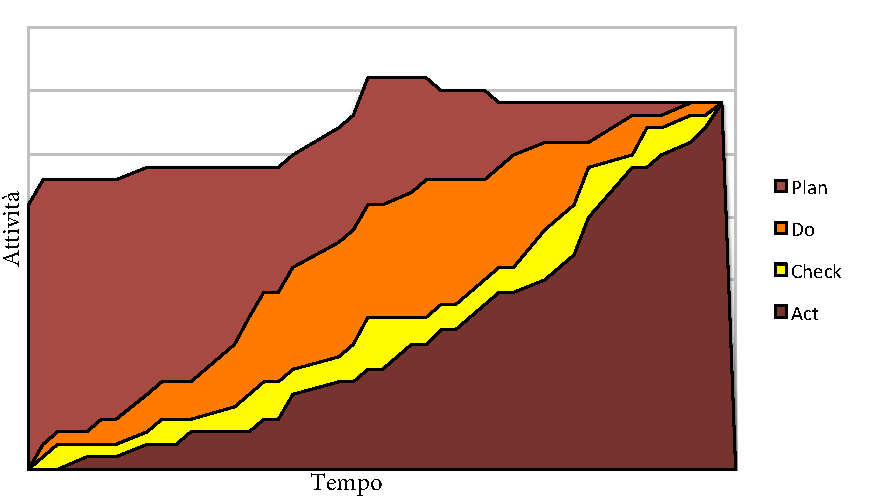
\includegraphics[width=\textwidth]{PianoDiQualifica/Pics/PDCAFaseA.pdf}
							\caption{PDCA Fase A}
						\end{figure}
						Guardando il grafico possiamo notare nella parte centrale un mutamento dei processi pianificati. Le cause di questa mutazione è l'inesperienza pianificazione e dei problemi nella creazione degli Use Case per il documento \insdoc{Analisi dei Requisiti}.\\
						Si può notare inoltre un lieve rallentamento nella parte finale causato dalla vicinanza della sessione di esami e quindi l'aumento degli impegni dei componenti del team.\\ \\
						
						